\begin{figure}
	\centering
	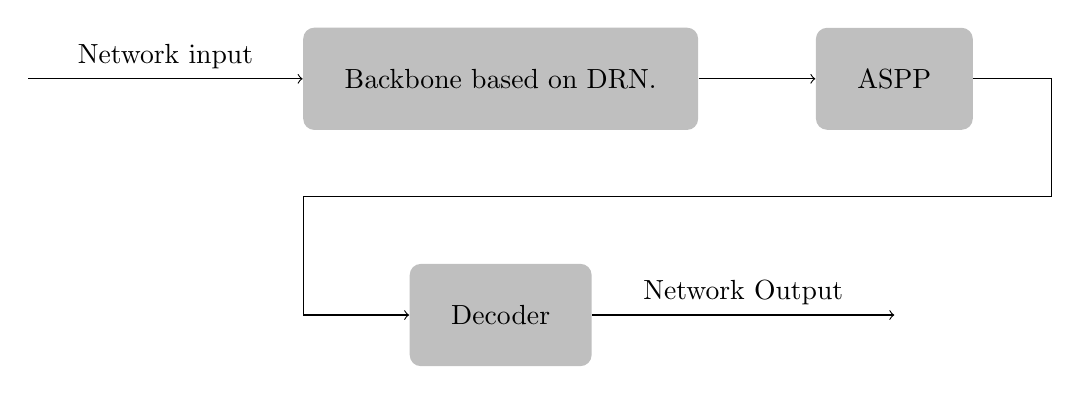
\begin{tikzpicture}
		% Backbone
		\node[fill=lightgray,rounded corners,inner sep=15pt] (backbone) at (0,0) {Backbone based on DRN.};
		% ASPP
		\node[fill=lightgray,rounded corners,inner sep=15pt] (ASPP) at (5,0) {ASPP};
		% Decoder
		\node[fill=lightgray,rounded corners,inner sep=15pt] (Decoder) at (0,-3) {Decoder};
		
		% Input arrow
		\draw [->] ++(-6,0) -- (backbone)
		node [above, midway] {Network input};
		% Backbone to aspp
		\draw [->] (backbone) -- (ASPP);
		% aspp to decoder
		\draw [->] (ASPP) -- (7,0) -- (7,-1.5) -- (-2.5,-1.5) -- (-2.5, -3) -- (Decoder);
		% Ouput arrow
		\draw [->] (Decoder) -- (5, -3)
		node [above, midway] {Network Output};

	\end{tikzpicture}
	\caption[Simplified Network Architecture]{A simplified visualization of the network architecture. The contents of each module is listed in Tables \ref{tab:drn}-\ref{tab:decoder}.}\label{fig:approach-network}
\end{figure}
